\documentclass[11pt]{article}
\usepackage[a4paper, margin=2cm]{geometry}
\usepackage[utf8]{inputenc}
\usepackage{amsmath}
\usepackage{amsfonts}
\usepackage{graphicx}\graphicspath{{images/}}
\usepackage{hyperref}
\usepackage{xcolor}

\begin{document}
\pagenumbering{gobble}

\begin{titlepage}
   \begin{center}
       \vspace*{6cm}

       \begin{large}\textbf{MXB326 Group Project - Reservoir Simulation}\end{large}

       \vspace{0.5cm}
        MXB326\_23se1 Computational Methods 2\\
        Due 26-05-2023
            
       \vspace{1.5cm}

       \textbf{Group 5: Benjamin Elliott, Christopher Deveney, Kye Miethke}

       \vfill
            
       MXB326\_23se1 Computational Methods 2\\
       Queensland University of Technology\\
       Semester 1 2023
            
   \end{center}
\end{titlepage}
\newpage

%================================== Outline ==================================%

\tableofcontents
\newpage
\pagenumbering{arabic}


\section{Introduction}
%================================== Introduction ==================================%
Oil is a natural resource which is used abundantly in modern society. Used in the creation of fuels which transport us around the world, to materials in products we use hundreds of times a day, and many places in between, it is no stretch to say that civilisation as we know it relies on oil. But the production of oil can be a slow and costly process. One method commonly used in the oil industry to improve production is called water-flooding. This processes uses the injection of water into the porous rock structure of an oil reservoir to increase the pressure, driving more oil out. Modelling this process mathematically is a key interest of a field of research known as reservoir engineering, and is of vital importance to ensure that the process of water-flooding runs smoothly.\\

This modelling, involving the simultaneous flow of two viscous fluids through a horizontal reservoir in three dimensions, is quite complex. Fortunately, the model can be substantially simplified when considering a homogeneous, one-dimensional reservoir. This simplification in turn reduces what would be a coupled system of partial differential equations into a single, one-dimensional PDE. To describe the mechanics of the system, the conservation of mass of oil and water assuming immiscibility and incompressibility, are given by the transport equations:
\begin{eqnarray}
\phi\frac{\partial S_w}{\partial t} + \frac{\partial q_w}{\partial x} = 0\\
\phi\frac{\partial S_o}{\partial t} + \frac{\partial q_o}{\partial x} = 0
\end{eqnarray}
In this system, $\phi$ indicates how porous the medium of the reservoir is, and $S_w$ and $q_w$, $S_o$ and $q_o$ indicate the saturation and flow rate of the water and oil respectively. We relate the pressure in each fluid as the capillary pressure: $P_c = p_o-p_w$, and assume that the capillary pressure is positive. Furthermore, the saturations of the oil and water can be related as $S_w +S_o = 1$, allowing a single saturation, $S=S_o$ to be the sole variable to be modelled. Also defined are the minimum, irreducible saturations $S_{or}$ and $S_{wr}$.\\

For a comprehensive description of the mathematical system, it is also necessary to define the conditions at the boundaries of the domain.
\begin{figure}[!h]
\centering
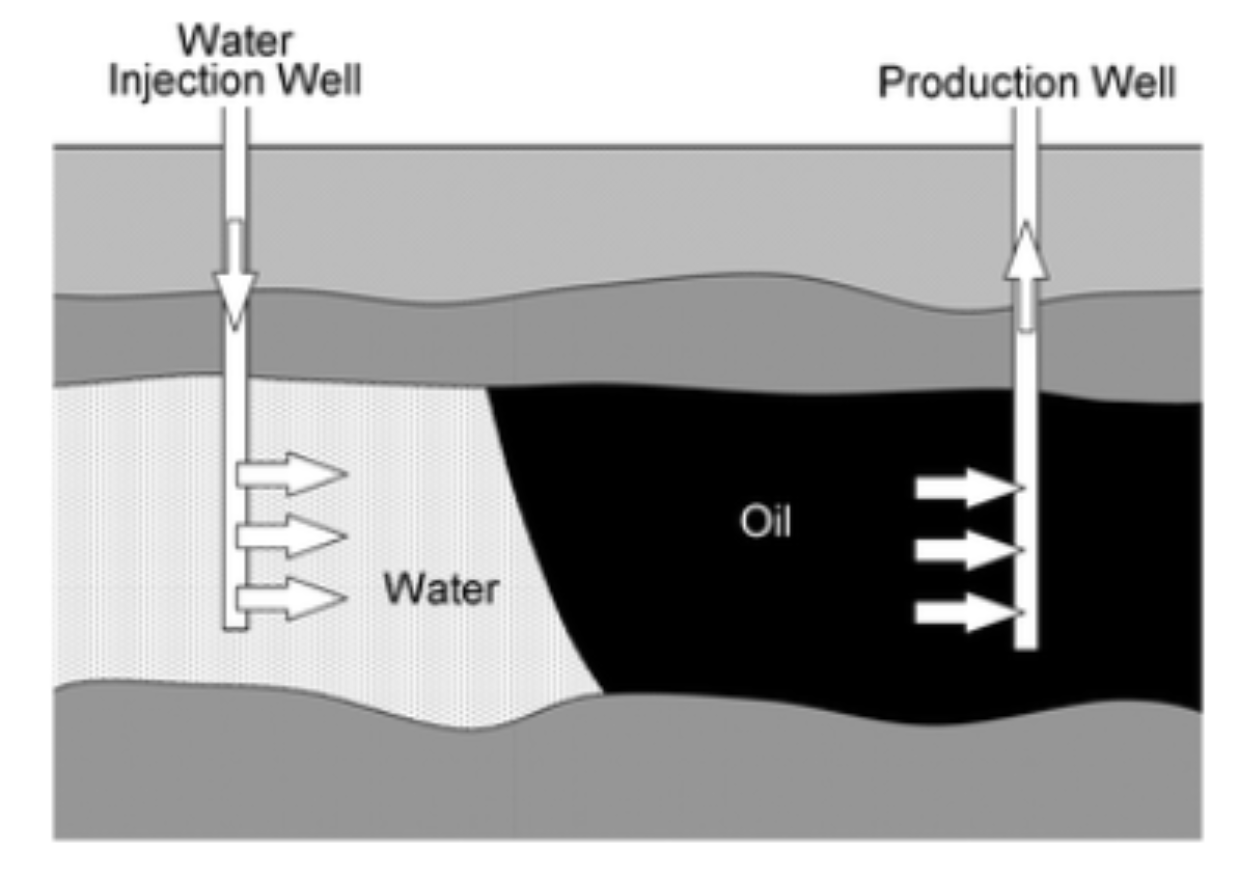
\includegraphics[width=0.4\textwidth]{injectionschematic.png}
\caption{Schematic of the oil injection process.}
\end{figure}
Figure 1 demonstrates the domain of the problem. Assuming a constant injection of water at $x=0$ at rate $q$:
\begin{eqnarray}
q_w(0,t) = q\\
q_o(0,t) = 0
\end{eqnarray}
And assuming oil saturation begins at its maximum value:
\begin{eqnarray}
S(x,0)=1-S_{wr}
\end{eqnarray}
Finally, assuming a semi-infinite reservoir:
\begin{eqnarray}
\lim_{x\to\infty} S(x,t) = 1-S_{wr}
\end{eqnarray}
For an efficient and cost-effective water-flooding operation, it is critical to prevent the water from mixing with the oil in the well-bore (extraction point). We thus define the breakthrough time as $T_B = 1-S_{or}-S_{wr}$, the time taken for the water to reach the well-bore during the water-flooding. Specification of a suitable injection rate $q$ is capable of preventing this issue from arising.\\

This report contains a pilot study of the simplified system above, including a mathematical model with a semi-analytic solution and a numerical solution. These solutions will be analysed thoroughly, with the goal of demonstrating the capability of a fully detailed study in the future. 
\smallbreak
\section{Mathematical Model}
%================================== Mathematical Model ==================================%

\smallbreak
\section{Semi-Analytical Solution}
%================================== Semi-Analytical Model ==================================%

\smallbreak
\section{Numerical Solution}
%================================== Numerical Solution ==================================%

\smallbreak
\section{Analysis and Findings}
%================================== Analysis and Findings ==================================%

\smallbreak
\section{Conclusions}
%================================== Conclusions ==================================%

\smallbreak
\section{References}
%================================== References ==================================%

\newpage
\end{document}
